\section{Grundlagen}

\subsection{Authentifizierung}
% TODO: Grundlagen der Authentifizierung (Definition, Verfahren, ...)
% Heutige Anwendungsbereiche und gängige Verfahren
% (Wo/Warum) wird Stimmauthentifizierung aktuell eingesetzt?
% Was wären mögliche Einsatzgebiete?
\subsection{Menschliche Stimme}


\subsubsection{Stimmerzeugung}
Die Stimmerzeugung unterteilt sich in zwei Phasen: die Phonation (Stimmbildung) und die Resonanz.
Bei der Phonation werden die Stimmbänder im Kehlkopf durch den Luftstrom in Schwingung versetzt, wodurch ein Ton (bestehend aus dem Grundton, sowie Obertönen) erzeugt wird.
Abhängig von der Spannung und Länge der Stimmbänder kann dabei die Tonhöhe des erzeugten Grundtons variiert werden.
Da sich der Kehlkopf bei Männern während des Stimmbruchs stärker vergrößert, liegt ihre Grundfrequenz tiefer \autocite[vgl.][S. 278-279]{clauss_humanbiologie_2018}.

Der erzeugte Grundton gelangt anschließend in den Vokaltrakt, bestehend aus dem Rachen-, Mund- und Nasenraum.
Dieser besitzt spezifische Resonanzeigenschaften, wodurch die Frequenzkomponenten des Grundtons verändert (verstärkt oder abgeschwächt) werden.
Durch die Artikulatoren Zunge, Lippen, Kiefer und Gaumensegel kann der Vokaltrakt und damit dessen Resonanzeigenschaften verändert werden.
Somit können die verschiedenen Laute, aus denen die Sprache aufgebaut ist, erzeugt werden \autocite[vgl.][S. 13-14]{pfister_sprachverarbeitung_2017}.

In der deutschen und englischen Sprache werden die Buchstaben des Alphabets grundlegend in Vokale und Konsonanten unterteilt.
Im folgenden werden die beiden Kategorien kurz erläutert.

\paragraph{Vokale}
Vokale zählen zu den stimmhaften Lauten.
Das bedeutet, dass hier die Stimmbänder im Kehlkopf einen Grundton erzeugen, welcher durch den Vokaltrakt verstärkt wird.
Die Luft kann dabei ungehindert durch den Mund ausströmen.
Die unterschiedlichen Vokale werden besonders durch die Position der Zunge und der Lippen gebildet \autocite[vgl.][S. 14]{pfister_sprachverarbeitung_2017}.

\paragraph{Konsonanten}
Im Gegensatz zu den Vokalen zeichnen sich Konsonanten dadurch aus, dass der Luftstrom teilweise oder vollständig durch eine Verengung behindert wird.
Die Verengung wird durch die Artikulatoren erzeugt.
Dabei gibt es sowohl stimmhafte, als auch stimmlose Konsonanten \autocite[vgl.][S. 15]{pfister_sprachverarbeitung_2017}.
% INFO: Hier könnte noch genauer auf stimmlose Konsonanten eingegangen werden -> z.B. was Grundfrequenz oder ähnliches angeht.

\subsubsection{Stimmwahrnehmung}
Im Gegensatz zu der Stimmerzeugung, lässt sich die Stimmwahrnehmung nicht ausschließlich anhand der Anatomie des menschlichen Ohrs erklären.
Deshalb werden in diesem Kapitel Eigenschaften der Stimme betrachtet, welche in Verbindung mit der Stimmwahrnehmung stehen.
Dazu zählen die Konzepte der Formanten und der Tonheit.
% TODO: Satz überarbeiten + gegebenenfalls Tonhöhen- und Lautstärkenwahrnehmung hinzufügen

\paragraph{Formanten}
Bei der Stimmerzeugung werden bestimmte Frequenzbereiche durch den Vokaltrakt verstärkt.
Diese Frequenzbereiche werden als Formanten bezeichnet und durch die Attribute (Mitten-)Frequenz, Bandbreite und Amplitude beschrieben.
Die Formanten werden in aufsteigender Frequenz angeordnet und mit $F_1, F_2, F_3 \dots$ bezeichnet.
Da die Formanten durch die Resonanzeigenschaften des Vokaltraktes erzeugt werden, sind diese besonders für die Erkennung von Vokalen relevant \autocite[vgl.][S. 19-20]{pfister_sprachverarbeitung_2017}.
Dabei ist die Position der Formanten sowohl von dem jeweiligen Vokal, als auch dem jeweiligen Sprecher abhängig.
% Besonders Vokale interessant -> stimmhaft + kontinuierlich/ungehindert, Formanten
% 
% INFO: Wichtig für Ausblick -> Bei Einsatz in Telefonie muss das Übertragungsspektrum berücksichtigt werden (kleiner als menschliche Stimme -> Verluste, ggf. von Grundfrequenz) => Schlechtere Qualität / Erkennung

\paragraph{Tonheit}
In der Psychoakustik unterscheidet sich die wahrgenommene Tonhöhe (auch Tonheit genannt) von der physikalischen Tonhöhe.
Die physikalische Tonhöhe wird durch die Grundfrequenz eines Tons bestimmt.
Eine Verdopplung der Grundfrequenz führt dabei zu einer Verdopplung der Tonhöhe.
Der Mensch nimmt jedoch diese Frequenzdifferenzen unterschiedlich wahr.
Während für geringe Frequenzen bis zu 500 Hz eine Ton mit doppelter Frequenz auch doppelt so hoch wahrgenommen wird, ist für Töne höherer Frequenz ein größerer Abstand notwendig.
Aus diesem Grund wurde im Jahr 1937 die Mel-Skala durch Stevens, Volkman und Newmann vorgeschlagen \autocite[vgl.][S. 11]{moser_psychoakustische_2018}.
Diese verläuft logarithmisch zur Frequenz, was auf den Aufbau der Basilarmembran im Innenohr zurückzuführen ist \autocite[vgl.][S. 54]{kroger_neuronale_2018}.
Als Bezug zwischen der Frequenz und der Mel-Skala wurde dabei die Frequenz 1000 Hz gewählt, welche 1000 mel entspricht.
Für die Umrechnung zwischen den beiden Skalen wird folgende Formel verwendet \autocite[vgl.][S. 94-95]{pfister_sprachverarbeitung_2017}:
\begin{equation}
    \label{eq:mel}
    h(f) = 2595 \cdot \log_{10}\left(1 + \frac{f}{700}\right)
\end{equation}

\subsection{Audioanalyse}
\subsubsection{Signalvorverarbeitung}
Um ein gegebenes Audiosignal einheitlich verarbeiten zu können, muss dieses zunächst mittels verschiedener Verfahren vorbereitet werden.
Ziel dieser Vorverarbeitung ist es, die Effizienz und Effektivität des anschließenden Verarbeitungsprozesses zu erhöhen und somit ein verbessertes Ergebnis zu erzielen \autocite[vgl.][S. 11672]{lokesh_speech_2019}.
Die Vorverarbeitung im Rahmen dieser Arbeit beinhaltet die vier Schritte Rauschreduzierung, Pausen entfernen, Framing und Windowing, welche im Folgenden genauer erläutert werden.

\paragraph{Rauschreduzierung}\label{sec:Rauschreduzierung}
Um störende Frequenzen aus dem Audiosignal zu entfernen, wird eine Rauschreduzierungsfunktion verwendet.
Die in dieser Arbeit verwendete Funktion nutzt den sogenannten Spectral Noise Gate Algorithmus.
Dabei wird zunächst die Signatur des Rauschens ermittelt.
Basierend darauf kann das Rauschen anschließend verringert werden \autocite[vgl.][S. 25]{kiapuchinski_spectral_2012}.

\paragraph{Pausen entfernen}
Die für die Sprecherauthentifizierung relevanten Daten stecken in dem aufgezeichneten Signal der Stimme.
Sprechpausen innerhalb des Audiosignals enthalten somit keine brauchbaren Informationen, weshalb diese herausgefiltert werden müssen.
Durch den vorangehenden Schritt der Rauschreduzierung kann hier ein stark vereinfachtes Verfahren gewählt werden.
Liegt das Signal für einen definierten Zeitraum unterhalb einer definierten Lautstärke, werden die entsprechenden Signalwerte aus dem Gesamtsignal entfernt.

\paragraph{Framing}\label{sec:Framing}
Für eine detaillierte Analyse des Audiosignals muss dieses in kleinere Blöcke unterteilt werden.
Dieser Prozess wird als Framing bezeichnet.
Dabei muss zunächst eine einheitliche Blockgröße festgelegt werden.
Da Stimmsignale aufgrund der Eigenschaften des Vokaltrakts über eine Periode von 10-30 ms stationär sind, wird eine Blockgröße in dieser Zeitordnung verwendet.
Zusätzlich wird eine Überlagerungszeit definiert, welche eine Überlappung der einzelnen Blöcke verursacht.
Durch die Überlappung wird ein Zusammenhang zwischen zwei benachbarten Frames und damit auch den anschließend berechneten Koeffizienten hergestellt \autocite[vgl.][S. 457]{richter_signal_2022}.

\paragraph{Windowing}
\begin{figure}
  \centering
  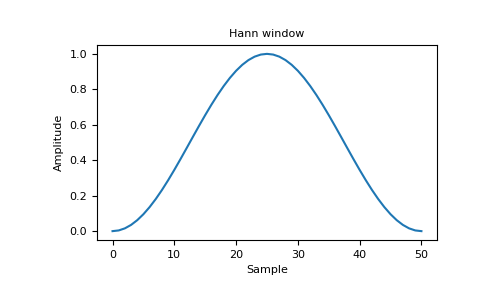
\includegraphics[width=0.8\textwidth, keepaspectratio]{images/hann_window.png}
  \caption{Von Hann Fensterfunktion \autocite{noauthor_numpyhanning_nodate}}
  \label{fig:vonHannFenster}
\end{figure}
Um die bei der Unterteilung des Audiosignals entstandenen Diskontinuitäten aufzulösen, wird eine Fensterfunktion auf die einzelnen Blöcke angewendet.
Abbildung~\ref{fig:vonHannFenster} zeigt die von Hann Fensterfunktion, welche neben dem Hamming Fenster zu den typischen Fensterfunktionen in der Audiosignalverarbeitung zählt.
Durch den Nulldurchgang am Anfang und Ende der Fensterfunktion werden die Amplituden des Blocksignals nach Anwenden der Funktion an den Grenzen auf Null gezogen, wodurch sich ein kontinuierlicher, periodischer Signalverlauf ergibt \autocite[vgl.][S. 462]{richter_signal_2022}.

Wird der Schritt des Windowing nicht durchgeführt, führt dies zu einem Phänomen namens spectral leakage.
Bei der Transformation des Signals von dem Zeitbereich in den Frequenzbereich resultiert der Amplitudensprung an den Blockenden in der Registrierung einer Vielzahl von Frequenzen.
Wie der Name bereits beschreibt, wird aus einer eindeutigen Frequenz, ein Spektrum aus Frequenzen, die nicht Teil des Signals sind \autocite[vgl.][S. 1296]{wu_new_2012}.

%%%% paste from t3000

\subsubsection{Fourier Analyse}

Jean-Baptiste Joseph Fourier (1768 - 1830) war ein französischer Mathematiker.
Er war in seinem Mathematikstudium Schüler von Lagrange, Laplace und Monge und veröffentlichte 1822 seine Arbeit \gqq{Theorie der Analytischen Funktionen}.
Damit legte er die Grundlagen für die Fourier-Reihe und die Fourier-Transformation.
Diese Verfahren sind bis heute in der Mathematik und Physik von großer Bedeutung und bilden die Grundlage für die Fourier-Analyse. Fourier gilt daher als einer der wichtigsten Mathematiker aller Zeiten \autocite[vgl.][o. S.]{heinz_klaus_strick_joseph_2012}.

Der Begriff Fourier-Analyse ist in der Literatur hauptsächlich für zwei Dinge verwendet worden.
Zum einen würdigt er die Rolle Fouriers in der Entwicklung der Mathematik.
Zum anderen ist er ein Überbegriff für eine Reihe an mathematischen Verfahren, die von Fourier entwickelt wurden \autocite[vgl.][S. 1]{picard_fourier-analyse_1996}.

\paragraph{Fourier-Reihe}

% Reihenentwicklung einer periodischen Funktion in Funktionsreihe aus Sinus- und Cosinusfunktionen

Die Fourier-Reihe ist ein Verfahren, mit dem eine periodische Funktion in eine unendliche Summe von Sinus- und Cosinusfunktionen zerlegt werden kann.
Wenn ein Signal $s(t)$ folgende Eigenschaften aufweist:

\begin{itemize}
    \item $s(t)$ ist periodisch mit der Periode $T$ (d.h. $s(t+T) = s(t)$)
    \item $s(t)$ ist stetig mit endlich vielen Sprungstellen im Intervall $[0,T]$
    \item $\int_{0}^{\infty} |s(t)| dt < \infty$
\end{itemize}

dann kann $s(t)$ in

\begin{equation}
s(t) = \frac{a_0}{2} + \sum_{n=1}^{\infty} a_n \cdot cos(n\omega_0t) + \sum_{n=1}^{\infty} b_n \cdot sin(n\omega_0t)
\end{equation}

zerlegt werden, wobei

\begin{equation}
a_0 = \frac{2}{T} \int_{0}^{T} s(t) dt
\end{equation}

\begin{equation}
a_n = \frac{2}{T} \int_{0}^{T} s(t) \cdot cos(n\omega_0t) dt
\end{equation}

\begin{equation}
b_n = \frac{2}{T} \int_{0}^{T} s(t) \cdot sin(n\omega_0t) dt
\end{equation}

\begin{equation}
\omega_0 = \frac{2\pi}{T}
\end{equation}

sind \autocite[vgl.][S. 19f]{ries_fourier-reihe_2018}.

Die Fourier-Koeffizienten $a_n$ und $b_n$ sagen also aus, wie stark einzelne Frequenzen in $s(t)$ vorkommen.
Diese Frequenzanteile sind als Output der Fourier-Reihe zu verstehen und können als Merkmale für periodische Signale verwendet werden.
$a_0$ ist der Mittelwert der Funktion $s(t)$.

\paragraph{Kontinuierliche Fourier-Transformation}

% Aperiodische Signale werden in kontinuierliches Spektrum zerlegt

Anders als bei der Fourier Reihe, können mit der verallgemeinerten kontinuierlichen Fourier-Transformation auch aperiodische Signale zerlegt werden, die folgende Eigenschaften aufweisen:

\begin{itemize}
    \item $s(t)$ ist stückweise stetig
    \item $\int_{-\infty}^{\infty} |s(t)| dt < \infty$
\end{itemize}

Die Fourier-Transformation liefert eine Transformierte Funktion $\underline{S}(f)$, die als Spektrum des Signals $s(t)$ bezeichnet wird.
Es wird also die Dimension Zeit $t$ in die Dimension Frequenz $f$ transformiert.
Die Formel für die Fourier-Transformation lautet:

\begin{equation}
    \underline{S}(f) = \int_{-\infty}^{\infty} s(t) \cdot e^{-j2\pi ft} dt
\end{equation}

Wie bereits an der Formel zu erkennen ist, ist das Ergebnis der Fourier-Transformation eine komplexe Funktion mit einem Realteil $\Re(\underline{S}(f))$ und einem Imaginärteil $\Im(\underline{S}(f))$.

Da bei der Weiterverarbeitung in der Regel nur der Normalteil des Spektrums benötigt wird, wird die Fourier-Transformation in der Praxis meistens in der Form

\begin{equation}
    \Re(\underline{S}(f)) = \int_{-\infty}^{\infty} s(t) \cdot cos(2\pi ft) dt
\end{equation}

durchgeführt \autocite[vgl.][S. 350f]{picard_fourier-analyse_1996}.

\paragraph{Diskrete Fourier-Transformation}

% Diskrete Signale werden in diskretes Spektrum zerlegt
Bei den bisherigen Analyseverfahren, wurden immer kontinuierliche Signale betrachtet.
Das heißt, dass für jeden Zeitpunkt $t$ ein Wert $s(t)$ existiert.

Bei der \ac{DFT} können diskrete Signale verarbeitet werden, die aus einer Folge von $N$ Werten ($s_0, s_1, \dots, s_{N-1}$) bestehen, weshalb diese Methode besonders interessant für elektronisch aufgezeichnete Signale ist.

Da keine kontinuierliche Funktion vorliegt, besteht keine Möglichkeit mehr, ein Integral zu bilden, weshalb die Formel jetzt mit einer Summe aufgestellt ist:

\begin{equation}
    S_k = \frac{1}{N} \sum_{n=0}^{N-1} s_n \cdot e^{-j2\pi \frac{kn}{N}}
\end{equation}

Der Output der \ac{DFT} ist wieder eine komplexe Wertereihe, deren Realteil $\Re(S_k)$ und Imaginärteil $\Im(S_k)$ die Amplitude und Phase der $k$-ten Frequenzkomponente des Signals $s_n$ beschreiben.
Der Realteil lässt sich durch die Umformung der Formel in die Form

\begin{equation}
    \Re(S_k) = \frac{2}{N} \sum_{n=0}^{N-1} s_n \cdot cos(2\pi \frac{kn}{N})
\end{equation}

berechnen \autocite[vgl.][S. 567ff]{smith_scientist_1997}.

Um auf die jeweiligen Frequenzanteile des Signals zu schließen, können die Output-Bins $S_k$ mit folgender Formel in die Frequenzen $f_k$ umgerechnet werden:
% TODO: Bins erklären

\begin{equation}
    f_k = \frac{k}{N} \cdot f_s
\end{equation}

wobei $f_s$ die Abtastrate des Signals ist.

\paragraph{Fast Fourier Transformation}

Die \ac{DFT} würde sich nach der obigen Formel implementieren und für jedes Signal nutzen lassen.
Allerdings ist die Komplexität der \ac{DFT} mit $\mathcal{O}(N^2)$ sehr hoch, weshalb die \ac{FFT} entwickelt wurde, die den gleichen Output liefert, aber mit einer Komplexität von $\mathcal{O}(N log(N))$ \autocite[vgl.][S. 338]{beucher_signale_2011}.

Die \ac{FFT} ist also eine für Computer optimierte Implementierung der \ac{DFT}.
Eine genaue Erklärung, warum \ac{FFT} signifikant weniger Berechnungen benötigt, würde für diese Seminararbeit zu sehr ins Detail gehen.
% TODO: Vlt doch ausführlich erklären
Einfach gesagt, nutzt der Algorithmus aber die Eigenschaft von Sinus- und Cosinus-Wellen, dass Wellen mehrfacher Frequenz an bestimmten Stellen dieselben Werte annehmen und so nur einmal berechnet werden müssen.

\begin{figure}
    \centering
    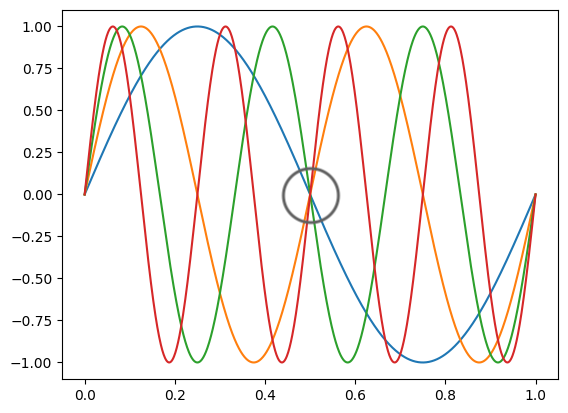
\includegraphics[width=0.5\textwidth]{images/fft-advantage.png}
    \caption{Sinuswellen mit 1hz, 2hz, 3hz, 4hz überlagern sich bei $t=0,5$}{Quelle: Eigene Darstellung}
    \label{fig:fft-advantage}
\end{figure}\noindent

Durch diese Eigenschaft und das rekursive Aufteilen des Signals in gerade und ungerade Datenpunkte spart der Algorithmus sehr viele Berechnungen ein \autocite[vgl.][S. 643]{oppenheim_discrete-time_1999}.

\newpage

\subsubsection{Mel Frequency Cepstral Coefficients}
Die \ac{DFT} ist durch das Herausfiltern der vorhandenen Frequenzen bereits gut geeignet, um wesentliche Merkmale, wie die Stimmlage und Stimmfarbe einer Aufzeichnung, zu bestimmen.
Allerdings werden in der Praxis meistens die \ac{MFCC} benutzt, die zwar auf einer Fourier-Analyse basieren, aber noch weitere Berechnungsschritte erfordern.

Der Vorteil von Merkmalen wie \ac{MFCC} ist zunächst, dass so Audio-Signale mit verschiedenen Längen und Abtastraten besser miteinander verglichen werden können.
Das liegt daran dass, bei einer Analyse der \ac{MFCC} eine feste Anzahl Koeffizienten entsteht.
Die Anzahl hängt dabei, anders als bei einer Fouriertransformation, nicht von der Frame-Länge und Abtastrate ab.
Zudem sind die \acp{MFCC} mehr auf die menschliche Wahrnehmung von Tönen abgestimmt und robuster gegenüber Hintergrundrauschen.

Um die Mel Frequency Cepstral Coefficients zu berechnen sind mehrere Schritte nötig \autocite[vgl. ][S. 2]{logan_mel_2000}:

\begin{enumerate}
    \item \textbf{Framing}\\Unterteilen des Signals 20 - 40 ms Abschnitte
    \item \textbf{\ac{DFT}}\\Bestimmung der Frequenzkomponenten
    \item \textbf{Logarithmierung}\\Näher an menschlicher Wahrnehmung
    \item \textbf{Abbildung auf die Mel-Skala\footnote{Das Mel ist eine Maßeinheit für die wahrgenommene Tonhöhe. Das Mel verläuft ab einer gewissen Frequenz logarithmisch und nicht mehr proportional zu Hertz, da ein Mensch die Tonhöhe logarithmisch wahrnimmt.}}\\Zusammenfassung von Frequenzen zu Mel-Bänder mithilfe von Dreiecksfiltern
    \item \textbf{Diskrete Kosinustransformation}\\Ähnlich zur inversen Fourier-Transformation
\end{enumerate}
%%%%
\subsubsection{Linear Predicitve Coding}
Die Grundlage von \ac{LPC} bildet das \ac{AR} Modell.
Die \ac{AR} basiert auf dem Konzept der multiplen Regression und wird auf zeitlich veränderliche Prozesse angewandt.
Dabei wird eine Kriteriumsvariable unter Betrachtung von einer beliebigen Anzahl an Prädiktorvariablen vorhergesagt \autocite[vgl.][S. 37-38]{canela_multiple_2019}.
Im speziellen Fall der \ac{AR} handelt es sich bei den Prädiktorvariablen um vorhergehende Werte des Prozesses.
Ein \ac{AR} Modell sagt somit den Wert zu einem Zeitpunkt $n$, basierend auf $p$ Vorgängerwerten des Prozesses voraus.
Es gilt somit der in Formel~\ref{eq:autoregression} dargestellte Zusammenhang, wobei $\hat{s}_n$ den vorausgesagten Wert, $s_{n-k}$ die vorhergehenden Werte, $a_{k}$ die Regressionsgewichte und $p$ die Anzahl an verwendeten Vorgängerwerten darstellt \autocite[][S. 1304]{atal_effectiveness_1974}.
\begin{equation}
  \hat{s}_{n} = \sum_{k=1}^{p} s_{n-k}a_{k}
  \label{eq:autoregression}
\end{equation}

Zur Bestimmung der Regressionsgewichte wurden verschiedene rekursive Verfahren entwickelt.
Neben der Yule-Walker Methode stellt der Burg Algorithmus eine beliebte Alternative dar, welcher in \citeauthor[][S. 443]{marple_new_1980} beschrieben ist.
% TODO: Formeln evtl. mit in die Arbeit ziehen
% Evtl: Formeln des Burg Algorithmus auflisten und erklären
% Evtl: Was hat Yule-Walker und Levinson damit zu tun?
\newline
\newline
Bei dem Verfahren \ac{LPC} wird der Ansatz verfolgt, Rückschlüsse von dem akustischen Signal auf die Stimmerzeugung zu ziehen.
Dazu wird ein \ac{AR}-Filter verwendet um ein vereinfachtes Modell des menschlichen Stimmtrakts zu erstellen.
Die Regressionsgewichte $a_k$ entsprechen dabei den \ac{LPC}-Koeffizienten.
% TODO: Genauer erklären warum die Gewichte eine Rolle spielen -> Stimmerzeugung mit Grundrauschen + Koeffizienten als Filter
\newline
\newline
Bei der Stimmerzeugung spielen die sogenannten Formanten eine Rolle.
Diese beschreiben die akustische Energie in einem unveränderlichen Frequenzbereich, welche wiederum von den Resonanz- und Interferenzeigenschaften des Artikulationsraums abhängen.
Dadurch werden bestimmte Frequenzen verstärkt, während andere gedämpft werden \autocite[vgl.][S. 259]{fitch_evolution_2000}.
Das durch die \ac{LPC}-Koeffizienten erstellte Modell erfasst die Resonanzeigenschaften des Signals, wodurch Rückschlüsse auf die Formanten geschlossen werden können.
Da die Struktur der Formanten sprecherspezifisch ist, kann der Sprecher somit über die \ac{LPC}-Koeffizienten identifiziert werden \autocite[vgl.][S. 117]{sidorov_text-independent_2010}.
\newline
\newline
Zur Berechnung der \ac{LPC}-Koeffizienten wird zunächst die selbe Annahme wie in Kapitel~\ref{sec:Framing} getroffen, dass sich die Form des Vokaltrakts und das in den Stimmritzen erzeugte Signal über den betrachteten Zeitraum nicht verändert \autocite[vgl.][S. 1304]{atal_effectiveness_1974}.
Somit lassen sich die Koeffizienten des \ac{AR}-Filters mittels des Burg-Algorithmus berechnen.

\subsection{Künstliche Intelligenz}
\ac{KI} hat in den letzten Jahren stark Aufmerksamkeit gewonnen und gilt als eine der wichtigsten Technologien des 21. Jahrhunderts.
Spätestens seit der Veröffentlichung und dem Erfolg durch den Chatbot ChatGPT am 30. November 2022 sind die Möglichkeiten von \ac{KI} den meisten Menschen bekannt. ChatGPT hat innerhalb von fünf Tagen die Schwelle von einer Million Nutzer erreicht. Spotify oder Facebook zum Vergleich haben hierfür 5 beziehungsweise 10 Monate benötigt \autocite[vgl. ][]{janson_infografik_2023}.
\newparagraph
Die Statistik die im Jahre 2022 vom IDC erstellt wurde prognostiziert für die Anwendungsfelder Hardware, Software und IT-Services im Jahre 2024 einen weltweiten Umsatz von 554,3 Milliarden US-Dollar.
Dies entspricht einer Steigerung von 171 Milliarden US-Dollar (44,6 \%) im Vergleich zum Jahr 2021 \autocite[vgl. ][]{idc_kunstliche_2022}.
Dies unterstreicht noch einmal die Relevanz von \ac{KI} im aktuellen Zeitalter.
Doch was ist \ac{KI} und wie ist Sie für diese Arbeit von Relevanz, diese Fragen werden im Folgenden beantwortet.
% ---- %
\newparagraph
Die Idee einer \acl{KI} ist bereits seit Mitte des 20. Jahrhunderts existent. 1955 definierte John McCarthy, einer der Pioniere der \ac{KI}, als erster den Begriff der \acl{KI} wie folgt:
\begin{quote}
  \gqq{Ziel der KI ist es, Maschinen zu entwickeln, die sich verhalten, als verfügten sie über Intelligenz.}
  \autocite[][S. 1]{ertel_grundkurs_2016}
\end{quote}\noindent
Aus heutiger Sicht ist diese Definition nicht mehr ausreichend.
Eine weit verbreitete Definition stammt von Elaine Rich die sagt, dass sich \ac{KI} mit der Entwicklung von Computeralgorithmen befasse, für Probleme, die Menschen im Moment noch besser lösen können \autocite[vgl. ][]{rich_artificial_1983}.
%Themenfelder KI
\newparagraph
Aufgrund der Entwicklung seit Mitte des 20. Jahrhunderts gliedert sich das Thema \ac{KI} in viele Teilgebiete.
% letztes Jahrzent vorallem Fortschritte im Bereich ML / grundsätzlich Lernen, welches relevant ist für Arbeit
Die verschiedenen Teilgebiete sind in der Abbildung \ref{fig:KI-Teilgebiete} dargestellt.
\begin{figure}[H]
    \centering
    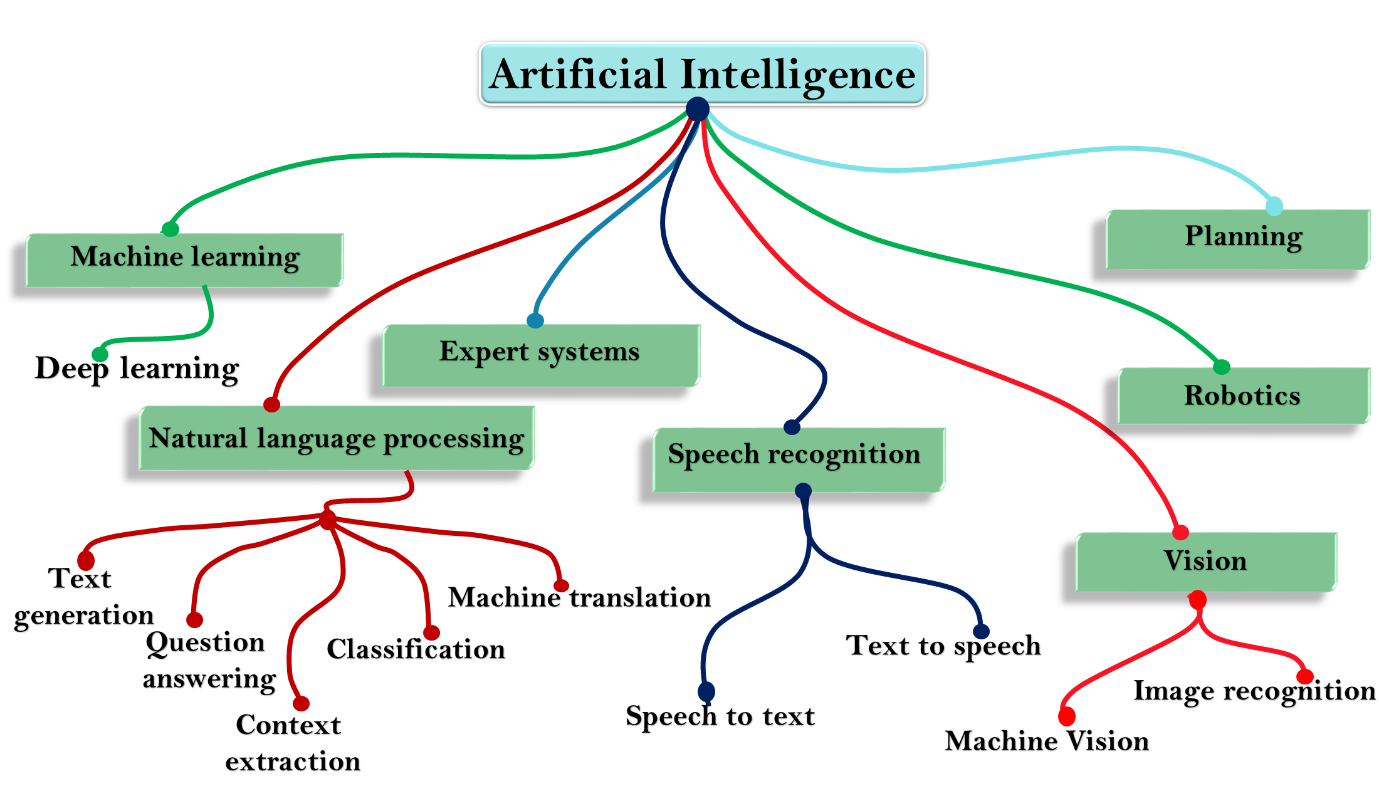
\includegraphics[width=0.9\textwidth]{images/KI_teilgebiete.png}
    \customcaption{Teilgebiete Künstliche Intelligenz}{\autocite[vgl.][]{noauthor_subsets_nodate}}
    \label{fig:KI-Teilgebiete}
\end{figure}\noindent
Insbesondere das Thema \ac{ML} hat in den letzten zehn Jahren viel Beachtung gefunden. 
\ac{ML} spielt für diese Studienarbeit eine entscheidende Rolle und wird deshalb im folgenden genauer betrachtet.
\newline
\ac{ML} ist nicht neu, bereits in den 1950er Jahren wurden von Arthur Lee Samuels die ersten \ac{ML} Programme entwickelt \autocite[vgl.][S. 5]{judith_hurwitz_machine_2018}.
Der Aufschwung von \ac{ML} im letzten Jahrzehnt ist auf steigende und bezahlbare Rechenleistung bzw. Speichergrößen zurückzuführen.
\ac{ML} beschreibt den Prozess bei dem Computeralgorithmen trainiert werden, um ihre Leistung bei einer bestimmten Aufgabe zu verbessern ohne das dies explizit programmiert werden muss.
Hierzu werden dem Computer Daten bereitgestellt aus welchen er lernt.
Der Computer kann anschließend aus den Daten gewonnenen Erkenntnisse nutzen, um Vorhersagen für neue Daten zu treffen \autocite[vgl.][S. 4]{judith_hurwitz_machine_2018}.
% Beispielsweise wird dem Computer eine Liste mit Häusern, deren Eigenschaften (z.B. Anzahl Zimmer, Wohnfläche, Alter und Standort) und einem Verkaufspreis zu Verfügung gestellt.
% Mit \ac{ML} wird ein Modell trainiert, das die Auswirkungen der Eigenschaften auf den Verkaufspreis analysiert.
% Dieses Modell kann verwendet werden, um den Verkaufspreis von anderen Häusern vorherzusagen.
Die Vorhersagen stimmen nicht immer zu 100 \%, die Vorhersagegenauigkeit hängt von verschiedenen Faktoren ab, welche je nach Anwendungsfall variieren.
\newline
\ac{ML} lässt sich in die drei Kategorien überwachtes Lernen, unüberwachtes Lernen und verstärkendes Lernen gliedern.
Beim überwachten Lernen besteht der Trainingsdatensatz aus Eingabewerten und gewünschten Ausgabewerten.
Der Algorithmus generiert eine Abbildungsfunktion, die die Eingabewerte auf die Ausgabewerte abbildet.
Der Computer wird sozusagen unterrichtet, Vorhersagen für zukünftige Daten auf Grundlage von Bestandsdaten zu erstellen \autocite[vgl][S. 11]{thakkar_beginning_2019}.
Im Gegensatz dazu besteht der Trainingsdatensatz beim unüberwachten Lernen nur aus unmarkierten Eingabewerten.
Das Ziel von unüberwachtem Lernen besteht darin Muster oder Strukturen zu erkennen.
Der Computer unterrichtet sich sozusagen selbst \autocites[vgl.][S. 11-12]{thakkar_beginning_2019}[vgl.][S. 6]{etaati_machine_2019}.
Verstärkendes Lernen ist ein verhaltensbasiertes Lernmodell.
Hierzu interagiert der Lernalgorithmus mit der Umgebung und erhält Belohnungen, wenn er die gewünschten Ergebnisse erzielt. 
Der Computer erlernt so das ideale Verhalten innerhalb der Umgebung \autocite[vgl][S. 12]{thakkar_beginning_2019}.

\subsection{Neuronale Netze}
In engem Zusammenhang zu \acl{ML} stehen die sogenannten \aclp{NN}.
Ein neuronales Netz ist ein maschinelles Modell, das auf dem Vorbild der Abläufe im Gehirn von Mensch und Tier basiert.
Durch geeignete mathematische Operationen wird versucht die Art und Weise abzubilden wie das menschliche Gehirn Probleme angeht beziehungsweise Zusammenhänge aus beobachten Daten erkennt \autocites[vgl.][S. 604]{backhaus_multivariate_2016}[vgl.][S. 31]{judith_hurwitz_machine_2018}.
Aus den vorhin genannten Lernalgorithmen (überwachtes, unüberwachtes, und verstärkendes Lernen) ergibt sich als Ergebnis ein neuronales Netz, welches das erlernte Wissen in seiner Struktur speichert \autocite[vgl.][S. 427]{guresen_definition_2011}.
\newparagraph
%Aufbau von neuronalen Netzen
Ein neuronales Netz ist prinzipiell in Schichten aufgebaut.
In jedem neuronalen Netz gibt es eine Eingabe- und Ausgabeschicht.
Zwischen der Eingabe- und Ausgabeschicht liegen mehrere versteckte Schichten (hidden layers).
Jede Schicht besteht aus mehreren Neuronen (Knoten), welche über gewichtete Kanten miteinander verbunden sind \autocite[vgl.][S. 26]{sonnet_neuronale_2022}.
Die Informationen werden durch die Neuronen in der Eingabeschicht aufgenommen und durch die Neuronen in der Ausgabeschicht ausgegeben.
Die Neuronen in der versteckten Schicht verarbeiten die Informationen.
Ein grundsätzlicher Aufbau eines neuronalen Netzes ist in Abb. \ref{fig:StructureNN} dargestellt.
\begin{figure}[H]
    \centering
    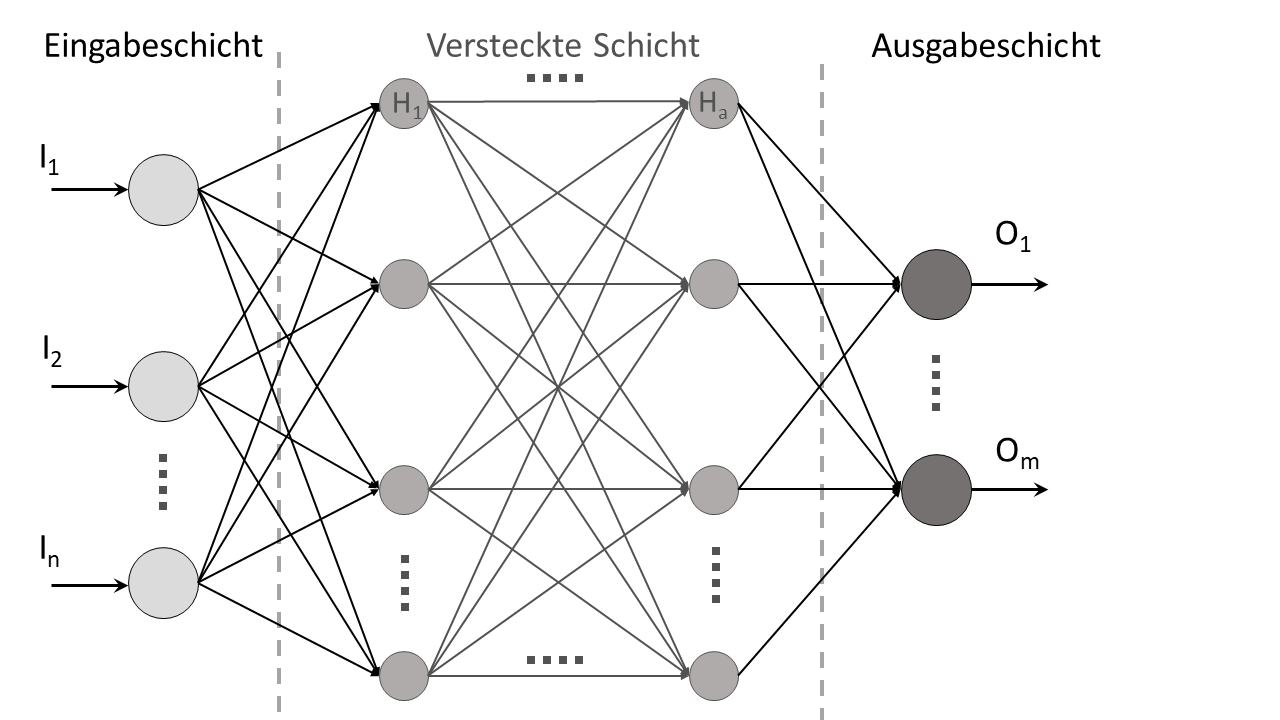
\includegraphics[width=0.9\textwidth]{images/structure_NN.png}
    \customcaption{Grundsätzlicher Aufbau eines neuronalen Netzes}{\autocite[][]{daniel_john_neuronales_2022}}
    \label{fig:StructureNN}
\end{figure}\noindent
Ein Neuron ermittelt seine Aktivierung aufgrund der Eingaben der vorherigen Neuronen und gibt daraus aufbauend einen Wert aus.
Dieser Wert kann durch die Gewichte auf den Kanten beeinflusst werden.
Von der Aktivierung ist abhängig, ob das Neuron feuert, sprich seinen errechneten Wert weitergibt.
Dies gibt Aufschluss über die Relevanz die vorangegangenen Werte.
% //TODO Quelle dazu suchen sonst \autocite[vgl.][S. 27]{sonnet_neuronale_2022}. beschreibt aber nut Aktivierung nicht was dies bedeutet
Somit können durch die Gewichte der Kanten und den Wert der Neuronen Informationen abgebildet werden.
\autocite[vgl.][S. 27]{sonnet_neuronale_2022}
\newparagraph
Für das Training von neuronalen Netzen werden viele klassifizierte Daten benötigt, welche als Ausgangspunkt dienen.
Das Training läuft iterativ in Schleifen, in sogenannte Epochen ab.
Nach jedem Durchlauf werden mithilfe des Feedbacks der Ausgabeschicht die Gewichte der Kanten und der Wert der Neuronen angepasst.
Zu Beginn werden die Kanten-Gewichte und der Wert eines Neurons zufällig gesetzt.
Dies wirkt sich auf das Ergebnis des gesamten Trainingsprozesses aus, da die zufällig gesetzten Werte so ungünstig sein können, dass das Netz während des Durchlaufs die Gewichte nicht ausreichend anpassen kann.
Nach Abschluss des Trainings kann das Netz bewertet werden.
Hierbei werden abhängig vom der gewählten Technologie unterschiedlich Parameter ausgegeben.
Grundsätzlich kann ein Netz immer beurteilt werden in dem bereits klassifizierte Daten, durch das Netz klassifizieren lässt und anschließend das Ergebnis das neuronale Netz mit dem tatsächlichen Ergebnis vergleicht.
Im Regelfall werden hierbei Daten genommen, welche zwar aus dem gleichen Datensatz stammen aber jedoch nicht für das Training genutzt wurden.
\autocite[vgl.][]{marcel_mikl_wie_2018}
% Arten von NN
